%!TEX root = ../physical-olympics-2.tex
\chapter{导体与介质}




\section{导体与静电平衡}

\subsection{绝缘体与导体}



微观地看,\,物质由原子或分子等组成,\,其中导电现象通常发生在不同情况下:

	\vspace{0.3cm}1. 真空导电:\,一般不会说真空具有\emph{导电性}(conductive),\,因为真空中是没有\emph{载流子}(charge carrier)的\footnote{量子场论认为真空存在电子对的产生湮灭涨落从而具有一定的导电性.}.\,的确,\,在\emph{阴极射线管}(cathode ray tube)中,\,加热一个阴极,\,并辅以合适的偏置电压可以造成真空中的电流.\,或是用一束能量足够的光子去轰击金属表面造成电子逸出,\,甚至纯粹由于阴极表面尖处十分强的电场导致电子直接克服逸出功发射出来.\,三种现象分别称为\emph{热发射}(thermionic emission),\,\emph{光电效应}(photoelectric effect)与\emph{场发射}(field emission).这种电荷的定向移动现象被统一地称为\emph{输运现象}(transport phenomenon).\,由于真空输运的独特性质,\,比如电子不会受到散射,\,平均自由程远大于仪器尺寸,\,与凝聚态物理中的一些概念对应,\,这被称为\emph{弹道输运}(ballistic transport).

	\begin{wrapfigure}[15]{o}[0pt]{5cm}
	\vspace{-2.2cm}
	\centering
	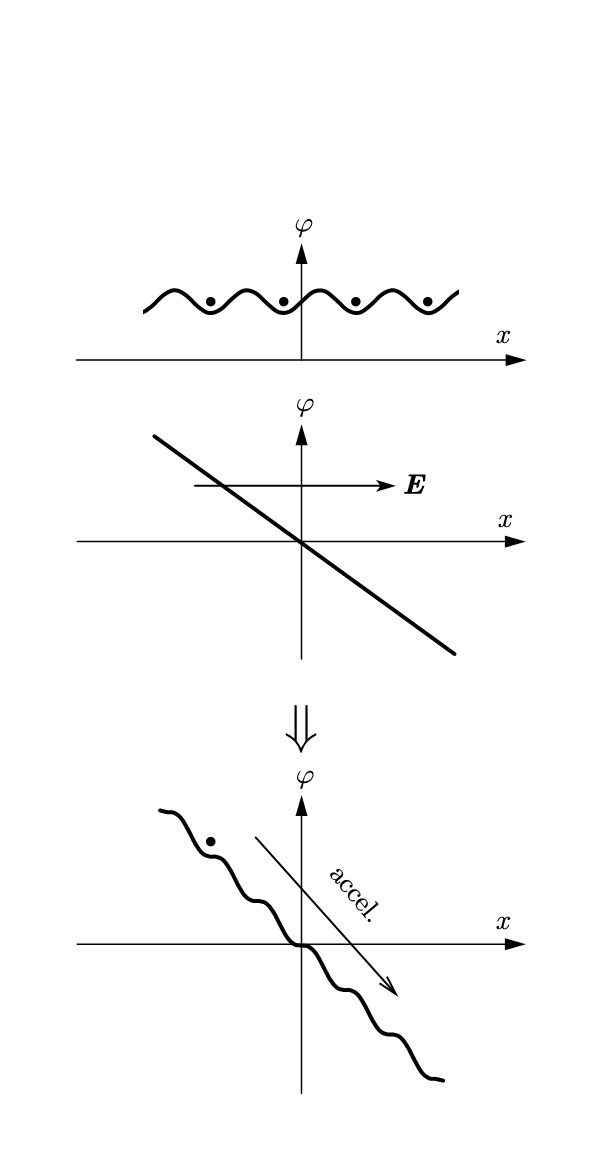
\includegraphics[width=5cm]{image/7-2-1.png}
	\caption{晶体击穿}
	\end{wrapfigure}

	\vspace{0.3cm}2. 绝缘体漏电:\,大多数非金属晶体,\,或是不含离子的液体与气体,\,原子核在晶体中都限制在点阵格子的特定位置,\,在气体,\,液体中则是可以活动的原子分子周围.\,电子分为两类,\,,一类是原子的内层电子,\,它极为稳定地存在于原子周围,\,离子晶体中的几乎完全被阴离子夺取的电子也属于这种情况.\,它们与原子核一起构成\emph{原子实}(atomic core).\,而\emph{价层电子}(valence shell electron),\,它们用来成键,\,将原子连接形成分子或者晶体,\,一般被定域在原子间的特定区域.\,所有这些电子的特点都是\emph{束缚态}(bond state).\,它们不能在介质中自由传导,\,一个电子的区域到另一个电子的区域间存在\emph{势垒}(potential barrirer),\,经典物理认为电子的动能不足以穿过这些势垒.\,但是,\,量子理论则认为电子的波函数可以通过\emph{隧道效应}(tunnelling)以小概率在不同区域间转移.\,这就为有电场的情况下电荷的平均定向移动提供了可能.\,这种现象称为\emph{漏电}(leakage).

	\vspace{0.3cm} 3. 绝缘体击穿:\,在十分高的电场下,\,原子与原子间,\,或是分子中显不同电性的部分之间的典型电压将大于阻碍电子转移的势垒.\,在晶体被击穿时此时电子在本质上可以被视为在周期性势能场与线性势能场的叠加中运动的经典粒子.\,不难看出电子不仅可以脱离单个势阱的束缚,\,还可以在这样的电场力下做持续的加速运动.\,气体液体则是在电场力作用下原子,\,分子被撕裂为离子而继续在电场力下做加速运动.\,此时碰撞就发生了:\,碰撞的结果往往是使得更多的原子分子发生电离.\,这样就会雪崩式的累积,\,固液气中的这些现象都称作\emph{雪崩击穿}(avalanche breakdown).\,尤其是气体中的放电现象在不同电流条件下分别造成\emph{汤森放电}(Townsend discharge),\,\emph{电晕放电}(corona discharge),\,\emph{辉光放电}(glow discharge),\,\emph{电弧放电}(arc discharge)的不同情况.

	\vspace{0.3cm} 4. 自然的导体:\,我们将材料区分为\emph{绝缘体}(insulator)与\emph{导体}(conductor),\,最重要的依据就是在弱场下是否天然地具有能产生电荷输运的载流子.\,所以导体就是一类事先就具有一定数密度$n$的一种或多种载流子$q$的材料,\,它们往往在有电场$\bs{E}$在场时发生位移,\,且与散射造成的形式阻力平衡,\,造成平均的匀速运动,\,即\emph{定向漂移}(directional drift).\,常见的金属以最外层的自由电子为载流子,\,半导体以热激发或掺杂形成的电子或空穴为载流子,\,电解质溶液或部分气态或液态的等离子体以阴阳离子为载流子.\,它们都是典型的导体.\,区别于前三种情况与最后的超导体.

	\vspace{0.3cm} 5. 超导体:\,低温下的很多奇异的宏观现象大大拓宽了人们对量子理论在物理学各个层次中应用的认识.\,其中很典型的一个就是\emph{超导}(superconductivity)现象.\,最早在1911年由\emph{昂内斯}({\it H. K. Onnes})在研究低温下汞的电阻率时惊人的发现在$4.2{\rm K}$下电阻率惊人地消失,\,这就是超导的发现.\,但是知道约十年后才引起足够重视.\,在$1933$年\emph{迈斯纳}({\it F. W. Meissner})才发现超导不仅仅是电阻率的消失,\,还伴随着\emph{完全抗磁性}(perfect diamagnetism):\,就好像理想导体内部无电场线,\,在超导体中交变的磁场也只能存在于表面极小的深度内(趋肤深度),\,也称迈斯纳效应.\,后来通过量子理论的蓬勃发展,\,在$1957$年提出的\emph{BCS理论}(Bardeen-Cooper-Schrieffer theory)终于解释了超导的成因,\,原来是一对\emph{库珀电子对}(Cooper pair)通过与声子(晶格振动)相互作用而造成了没有任何散射的量子模式.\,完整地解释了直到1986年所有\emph{低温超导}(low-temperatre superconductivity)的现象.\,但是随着$35{\rm K}$超导的镧钡铜氧体的发现,\,宣告人类进入\emph{高温超导}(high-temperatre superconductivity)纪元.\,新的超导材料不断被发现,\,新的理论也不断被提出,\,目前最``高温"的材料是汞钡钙铜氧体,\,超导临界温度$135{\rm}$.\,为什么有高温超导?\,高温超导的临界温度如何进一步提高?\,直到今天这也还是方兴未艾的研究领域.\,其在科研,\,科技,\,生产,\,生活方面的应用是不可估量的.

\vspace{0.5cm}

我们将把研究的范围主要放在导电的导体和不导电的绝缘体上.\,前者分析其静电平衡,\,即本章的内容;\,稳恒电流,\,下一章的内容;\,和之后章节的拟稳的一些情况.\,对于绝缘体我们本章也介绍其介电特性,\,光作为电磁波在其中的传播则放到光学中讲解.

\subsection{导体的特点}

这里说的导体,\,主要指固体形式的金属.

首先界定我们研究的问题范围:\,\emph{静电平衡}(electrostatic equilibrium)问题是一种\emph{稳态}(steady state).\,我们研究的问题由各式各样的,\,有限的块状导体${\rm C}_1,\,{\rm C}_2\cdots {\rm C}_n$构成,\,这些导体带电情况由体电荷密度$\rho$和面电荷密度$\sigma$描述.\,但是导体${\rm C}_i$上的总电荷量不一定为零:
\[Q_i=\int\limits_{{\rm C}_i}\rho \ud V+\int\limits_{\partial{\rm C}_i}\sigma \ud S\neq 0\]

这个电量$Q_i$一般也是可以在一定范围内人为控制的,\,即给导体\emph{充电}(charge).\,利用电容的性质很容易可以做到这一点.\,在为导体充电后由于电量守恒,\,其总电量就不能改变了,\,但是其电荷分布一般是未知的.


除了它们往往还有人为指定的各种点电荷$q_j$或者电荷分布$\rho(\bs{r})$存在于导体外.\,那么,\,容易想像,\,当导体外突然产生电荷分布时(如原来中和的电荷被重新分开),\,或者导体被置入电荷体系中,\,本质上就是当导体外的场环境发生改变时,\,导体内部显然不可能保持电场强度始终为零.\,只要有电场就会引起电流,\,它必然使得内部和表面的电荷分布发生改变$\dot{\rho}(t),\,\dot{\sigma}(t)\neq 0$.\,这些状态就是\emph{暂态}(transient state).\,但是只要外界的场不再变动,\,经过特征的\emph{弛豫时间}(relaxation time)后,\,一般很短只有$10^{-14}{\rm s}$量级,\,就会接近直到变成稳态.

通过以上推理,\,足以看出,\,静电平衡下,\,导体内部应当没有电场.\,这就是静电平衡理论的初始命题.\,它的初步推演泛化出以下的九宫格式的结论,\,分别讨论导体内,\,导体表面,\,导体外三处的电荷分布,\,电场分布,\,和电势分布三个特性:

\begin{table}[H]
\centering
\begin{tabular}{|c||c|c|c|}
\hline
一般特征	&电荷		  		&电场&电势\\
\hline\hline
导体内 		&$\rho = 0$			&$\bs{E} = 0$	&$\varphi=C$\\
\hline
导体表面	&$\sigma\neq 0$ 	&奇异			&$\varphi=C$\\
\hline
导体外 		&$\rho \neq 0$ 	&$\bs{E} \neq 0$&$\varphi\neq C$\\
\hline
\end{tabular}
\caption{静电平衡的初级结论}
\end{table}

其实就是说,\,因为导体内部没有电场,\,所以导体内部也没有形成电场的电荷(高斯定理可证),\,也使得导体成为一个\emph{等势体}(equipotential body),\,导体表面成为一个\emph{等势面}(equipotential surface).\,注意,\,这里说的``内部'',\,``表面'',\,``外部"包含两种情况.\,导体内部就是金属成分的空间,\,外部一般是真空与外加电荷分布的空间,\,表面是它们的分界面,\,但是下图的第一种情况,\,导体的外部延伸到了无穷远,\,这种为\emph{开外界}(open exterior),\,但是后两种情况,\,导体的外部是有限的\emph{闭外界}(closed exterior).\,第二种典型情况这个单连通的闭外界还被称作\emph{空腔}(cavity).\,除非特殊说明,\,我们一般默认导体的内部不会延伸到无穷远.

\begin{figure}[H]
\centering
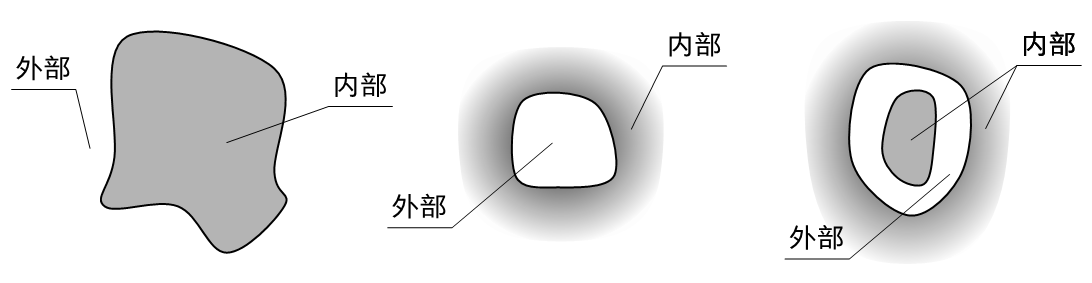
\includegraphics[width=0.7\textwidth]{image/7-2-2.png}
\caption{导体内外}
\end{figure}

在导体表面发生了电场计算的奇异性,\,因为这里是面电荷分布.\,我们考察细节就会进一步发现以下进一步的结论:\,导体表面的面电荷只朝外侧发出电场线,\,其方向垂直于表面(电场线垂直于等势面),\,且疏密程度正比于电荷密度(即高斯定理):
\[\bs{E}=-\nabla\varphi=\frac{\sigma}{\varepsilon_0}\bs{n}\]

\begin{figure}[H]
\centering
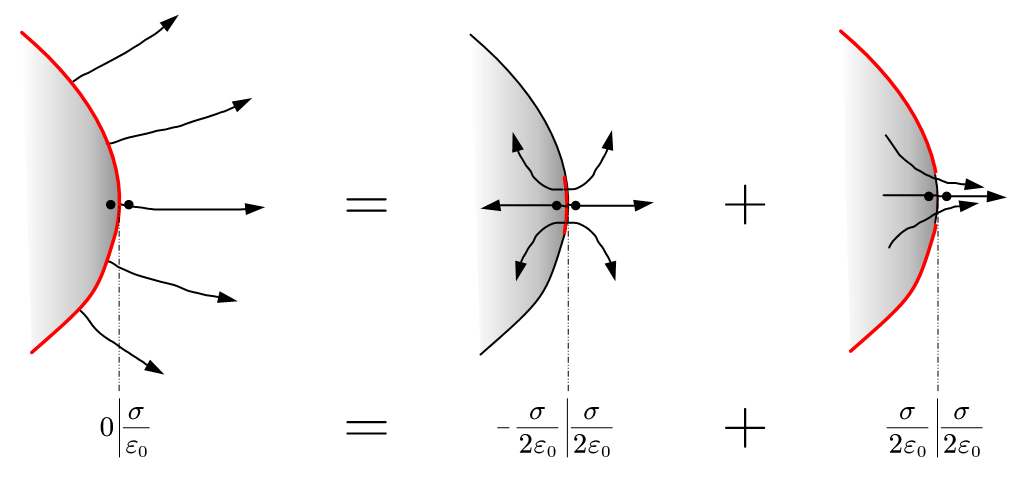
\includegraphics[width=0.6\textwidth]{image/7-2-3.png}
\caption{导体表面}
\end{figure}

但是正如上图所示,\,如果在十分接近表面的内外各取一点,\,就会发现如果只选取相对这两点足够大的一块面电荷(但又足够小以至于可以视作平面),\,它对面左右的电场强度只贡献以上值的一半.\,那么另一半必然由去掉这一块电荷的另外的部分所贡献.\,所以如果要讨论面上的场强,\,通过上一节的主值积分的理解方式,\,它就自然地被定义为内外场强和的一半,\,即:
\[\bs{E}=\frac{\sigma}{2\varepsilon_0}\bs{n}\]

对于导体静电平衡问题的计算求解,\,也包括模拟求解,\,本质上都建立在以下基本原理的基础上:

\begin{verse}
\emph{独立叠加原理}:\,静电平衡问题可以拆解为一个个独立的在导体外部连通区域的静电边值问题.
\end{verse}

所谓的\emph{边值问题}(boundary value problem)本是偏微分方程的术语,\,在这里特指下面说的静电情况.\,每一种情况中,\,我们无需分析导体的内部的电荷,\,电场,\,电势.\,只需要求解外部的电场$\bs{E}(\bs{r})$和电势$\varphi(\bs{r})$.\,导体外部的电荷分布$\rho(\bs{r})$却是事先给定的.\,还已知的是每一种导体表面的,\,要么是电势$\varphi_i$(从而导体内部的电势也是这个值),\,把这种导体称作第一类导体,\,对应条件称为第一类边界条件;\,要么是已知这个面上的总电量$Q_i$,\,把这种导体称作第二类导体,\,对应条件称为第一类边界条件.\,而每一个导体外部的区域的边界,\,就回到了各个导体的表面$\Sigma_1,\,\Sigma_2\cdots\Sigma_n$构成的集合.\,但是表面上的电荷分布也是事先不知道的.\,由于电荷,\,电场都可以从电势中得到,\,故只暂时考虑求电势,\,我们把静电边值问题整理一下:

\begin{verse}
\emph{已知}:\,导体外连通区域$D$以第一类导体表面$\Sigma_1,\,\Sigma_2\cdots\Sigma_n$和第二类导体表面$\Pi_1,\,\Pi_2\cdots\Pi_m$为边界.\,已知区域$D$内电荷分布$\rho$,\,已知第一类导体表面$\Sigma_i$上的电势$V_i$.\,已知第二类导体表面$\Pi_j$上的电量$Q_j$:
\[\partial D=\biggl(\bigcup_i \Sigma_i\biggr)\cup \biggl(\bigcup_j\Pi_j  \biggr) \]
\[\rho=\rho(\bs{r}) \quad,\quad \bs{r}\in D\]
\[\varphi(\bs{r})|_{\Sigma_i}=V_i \quad, \quad \int\limits_{\Pi_j}\nabla\varphi\cdot \ud \bs{S}=Q_j \quad, \quad \varphi(\bs{r})|_{\Pi_j}=C\]

\emph{未知}:\,导体表面电荷的具体分布$\sigma(\bs{r})|_{\Sigma_i,\,\Pi_j}$

\emph{待求}:\,$D$内的电势分布$\varphi(\bs{r})|_{D}$

\end{verse}


\begin{wrapfigure}[11]{o}[0pt]{7cm}
\vspace{-0.2cm}
\centering
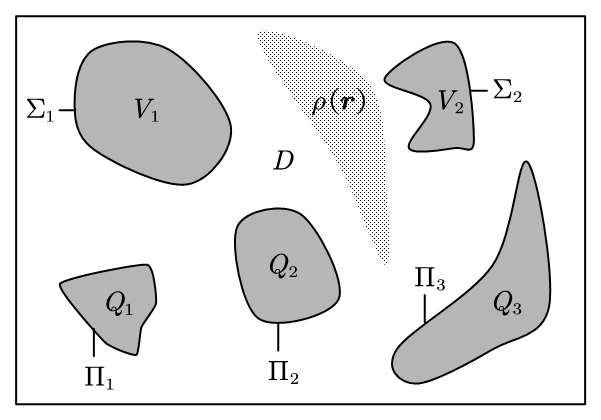
\includegraphics[width=7cm]{image/7-2-4.png}
\caption{边值问题}
\end{wrapfigure}
但是还要注意这种边值问题又分为\emph{外问题}(outside problem)和\emph{内问题}(inside problem)两类.\,外问题是区域$D$延伸到了无穷远,\,这种情况的边值问题提法就完全如上所述.\,但是内问题中区域$D$存在一个最外的表面$\Sigma_0$,\,它把整个$D$和其他所有金属表面与内部包含在其内部.\,$\Sigma_0$的外部亦是金属.\,对于内问题,\,我们很容易发现$\Sigma_0$上的总带电量为内部所有带电量的和的相反数,\,且仅仅由内部体系和它产生的电场线不会延伸到$\Sigma_0$外部.\,所以我们可以规定这一类问题中$\Sigma_0$上的电势为$0$:
\[\varphi(\bs{r})|_{\Sigma_0}=0\]

而其他所有第一类导体的电势皆是相对它而言的电势差.

\begin{wrapfigure}[10]{o}[0pt]{7cm}
\vspace{-0.2cm}
\centering
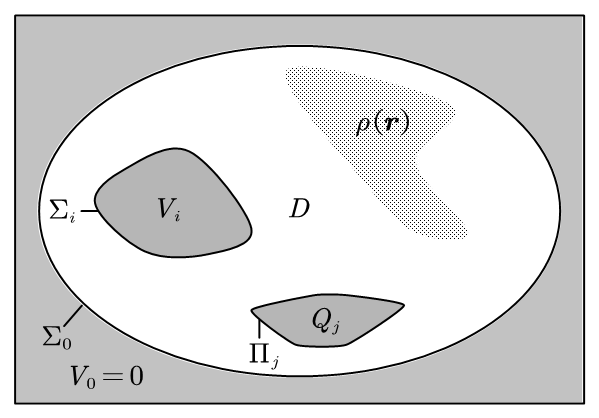
\includegraphics[width=7cm]{image/7-2-5.png}
\caption{内问题}
\end{wrapfigure}
对于每一个具体的边值问题,\,指导我们求解的重要思想是\emph{广义叠加原理}(general superposition principle)和\emph{唯一性定理}(uniqueness theorem).\,从语义上看广义叠加原理显然与之前的单纯的叠加原理有着直接的联系.\,其实它更是来自于数学上具有线性结构的系统的解的叠加原理.\,这个叠加原理是这样表述的:
\begin{verse}
\emph{广义叠加原理}:\,两个边值问题如果$D,\,\Sigma_i,\,\Pi_j$一致.\,第一个问题具有第一类边界条件$V_{1i}$和第二类边界条件$Q_{1j}$和内部电荷分布$\rho_1(\bs{r})|_D$.\,第二个问题具有第一类边界条件$V_{2i}$和第二类边界条件$Q_{2j}$和内部电荷分布$\rho_2(\bs{r})|_D$.\,两个问题的解分别为$\varphi_1(\bs{r})|_D,\,\varphi_2(\bs{r})|_D$.\,则同样以$D$为区域,\,$\Sigma_i,\,\Pi_j$为$D$两类导体边界,\,但是以$V_{1i}+V_{2i}$和$Q_{1j}+Q_{2j}$为两类边界条件的问题的解一定是:
\[\varphi(\bs{r})=\varphi_1(\bs{r})+\varphi_2(\bs{r})\]
\end{verse}

这个定理的证明是显然的.\,首先对于一个边值问题的解$\varphi$,\,它只需要满足以下一个全局条件和之前的边值条件:
\[\nabla^2\varphi=-\frac{\rho}{\varepsilon_0}\]
\[\varphi(\bs{r})|_{\Sigma_i}=V_i \quad, \quad \int\limits_{\Pi_j}\nabla\varphi\cdot \ud \bs{S}=Q_j \quad, \quad \varphi(\bs{r})|_{\Pi_j}=C\]

那么既然$\varphi_1$和$\varphi_2$都是之前两个问题的解,\,这就意味着:
\[\nabla^2\varphi_1=-\frac{\rho_1}{\varepsilon_0} \quad,\quad \nabla^2\varphi_2=-\frac{\rho_2}{\varepsilon_0}\]
\[\varphi_1(\bs{r})|_{\Sigma_i}=V_{1i} \quad, \quad \int\limits_{\Pi_j}\nabla\varphi_1\cdot \ud \bs{S}=Q_{1j} \quad, \quad \varphi_1(\bs{r})|_{\Pi_j}=C\]
\[\varphi_2(\bs{r})|_{\Sigma_i}=V_{2i} \quad, \quad \int\limits_{\Pi_j}\nabla\varphi_2\cdot \ud \bs{S}=Q_{2j} \quad, \quad \varphi_2(\bs{r})|_{\Pi_j}=C\]

那么定义$\varphi=\varphi_1+\varphi_2$,\,它就自然也能满足:

\[\nabla^2\varphi=-\frac{\rho_1+\rho_2}{\varepsilon_0}\]
\[\varphi(\bs{r})|_{\Sigma_i}=V_{1i}+V_{2i} \quad, \quad \int\limits_{\Pi_j}\nabla\varphi\cdot \ud \bs{S}=Q_{1j}+Q_{2j} \quad, \quad \varphi(\bs{r})|_{\Pi_j}=C\]

从而就的确是原来的问题的一个解.\,但是这个解是否唯一?\,答案是肯定的.\,这就是著名的唯一性定理,\,可以这么表述:
\begin{verse}
\emph{唯一性定理}:\,如果同一个边值问题具有两个解$\varphi_1,\,\varphi_2$.\,那么$\varphi_1-\varphi_2= 0$.
\end{verse} 	 

其证明的核心思想是利用上一章介绍的第一格林等式\footnote{其实使用简单的``电荷发出电场线,\,沿电场线方向电势降低"的观点也是可以论证这个定理的.}.\,首先注意到如果$\varphi_1,\,\varphi_2$都是同一个边值问题的解.\,那么命$\varphi=\varphi_1-\varphi_2$就是以下边值问题的解:
\[\nabla^2\varphi=-\frac{\rho-\rho}{\varepsilon_0}=0\]
\[\varphi(\bs{r})|_{\Sigma_i}=0 \quad, \quad \int\limits_{\Pi_j}\nabla\varphi\cdot \ud \bs{S}=0 \quad, \quad \varphi(\bs{r})|_{\Pi_j}=C\]

上面这个等号右侧都是零的方程称作\emph{齐次方程}(homogeneous equation).\,那么问题就被转化为证明齐次方程的解必为零解.\,想起第一格林等式:
\[\nabla\cdot(\phi\nabla\psi)=\phi\nabla^2\psi+\nabla\phi\cdot\nabla\psi\]

同样是在$\phi,\,\psi$都取$\varphi$的情况:
\[\varphi\nabla^2\varphi=\nabla\cdot(\varphi\nabla\varphi)-(\nabla\varphi)^2\]

现在把$\varphi$就视作刚刚定义的$\varphi_1-\varphi_2$,\,并把这个公式运用于$D$中的任意一点,\,由于电势满足的条件$\nabla^2\varphi=0$,\,就有:
\[(\nabla\varphi)^2=\nabla\cdot(\varphi \nabla\varphi)\]

等号右侧会让人联想到奥-高定理.\,事实上如果把它应用到$D$:\,左右两侧就能化为:
\[\int\limits_D(\nabla\varphi)^2\ud V=\int\limits_D \nabla\cdot(\varphi \nabla\varphi)\ud V=\oint\limits_{\partial D}\varphi\nabla\varphi \cdot \ud \bs{S}=\oint\limits_{\scriptscriptstyle\left(\cup_i \Sigma_i\right)\cup \left(\cup_j\Pi_j  \right)}\cdots=\sum_i \oint\limits_{\Sigma_i}\varphi\nabla\varphi \cdot \ud \bs{S}+\sum_j \oint\limits_{\Pi_j}\varphi\nabla\varphi \cdot \ud \bs{S}\]

在第一类导体边界上,\,由于$\varphi=0$所以积分为零.\,在第二类导体边界上,\,首先$\varphi$也是常数所以可以提出到积分外面,\,即:
\[\oint\limits_{\Pi_j}\varphi\nabla\varphi \cdot \ud \bs{S}=C\cdot\oint\limits_{\Pi_j}\nabla\varphi \cdot \ud \bs{S}=C\cdot 0=0\]

从而得到恰好等号的右侧就是$0$.\,这就相当于证明了这个电势$\varphi$满足:
\[\int\limits_D(\nabla\varphi)^2\ud V=0\]

一个总是不小于零的$(\nabla\varphi)^2$,\,经过积分得到了零的结果.\,这就说明它恒等于零:
\[\nabla\varphi=\bs{0}\]

从而电势就是一个常数,\,由于在第一类边界条件上得取零,\,故只能是:
\[\varphi=0\]

\vspace{1cm}

利用以上两个原理,\,在区域$D$是高度对称的条件下,\,在外加上内部没有电荷分布$\rho$的条件下.\,足以解决很多实际的问题:\,下面举一些频繁使用的例子:

\subsection{常见简单体系}

\subsubsection{1.\,平行的无限大导体板}
我们先考虑无限大的导体平面板,\,它可能具有一定的厚度.\,把这样的$n$块板子从左至右平行放置,\,如图\ref{fig7-2-6}.\,这样就把空间隔离为中间的$D_{12},\,D_{23},\,\cdots,\,D_{n-1\,n}$等区域.
\begin{wrapfigure}[10]{o}[0pt]{7cm}
\vspace{-0.2cm}
\centering
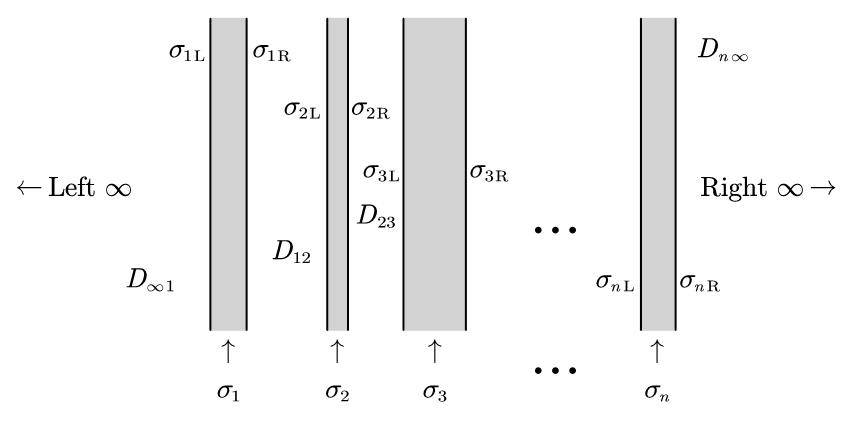
\includegraphics[width=7cm]{image/7-2-6.png}
\caption{平行板问题}\label{fig7-2-6}
\end{wrapfigure}
不同于上一节介绍的严格边值问题的提法.\,我们没有必要严格的讨论在某些边值条件下这个问题的解.\,仅仅把这种情况下体系需要满足的性质罗列出来.\,首当其冲地当属每一块板上的电量需要满足的关系.\,如果板非常薄,\,那么左右两侧的带电面密度$\sigma_{i{\rm L}}$和右侧

\subsubsection{2.\,同心导体球与球壳}

\subsubsection{3.\,共轴的导体圆柱与圆柱壳}


\section{电像法}

\section{电介质}

\section{再议静电能}
